\documentclass[12pt,compress,ngerman,utf8,t]{beamer}
\usepackage{etex}
\usepackage{ragged2e}
\usepackage[ngerman]{babel}
\usepackage{calc,dashrule,tabto,tikz}
\usetikzlibrary{arrows}
\usepackage[protrusion=true,expansion=true]{microtype}
\usepackage[normalem]{ulem}

\graphicspath{{images/}}

\title[Unendlich große Zahlen]{\bf Die wundersame Welt der \\ unendlich großen Zahlen}
\author[Ingo Blechschmidt]{\textcolor{white}{Gymnasium Königsbrunn \\ Abend der
Mathematik \\ 2. Juli 2019}}
\date[2019-07-02]{\vspace*{6em}\ \\\textcolor{white}{Ingo Blechschmidt \\ \scriptsize
Università di Verona \\}}

\useinnertheme[shadow=true]{rounded}
\useoutertheme{split}
\usecolortheme{orchid}
\usecolortheme{whale}
\setbeamerfont{block title}{size={}}

\useinnertheme{rectangles}

\usecolortheme{seahorse}
\definecolor{mypurple}{RGB}{150,0,255}
\setbeamercolor{structure}{fg=mypurple}
\definecolor{myred}{RGB}{150,0,0}
\setbeamercolor*{title}{fg=white}
\setbeamercolor*{titlelike}{bg=myred,fg=white}

\usefonttheme{serif}
\usepackage[T1]{fontenc}
\usepackage{libertine}

\setbeamertemplate{navigation symbols}{}

\setbeamertemplate{title page}[default][colsep=-1bp,rounded=false,shadow=false]
\setbeamertemplate{frametitle}[default][colsep=-2bp,rounded=false,shadow=false,center]

\newcommand{\hil}[1]{{\usebeamercolor[fg]{item}{\textbf{#1}}}}
\setbeamertemplate{frametitle}{%
  \vskip1em%
  \leavevmode%
  \begin{beamercolorbox}[dp=1ex,center]{}%
      \usebeamercolor[fg]{item}{\textbf{\textsf{\Large \insertframetitle}}}
  \end{beamercolorbox}%
}

\setbeamertemplate{headline}{}
\setbeamertemplate{footline}{%
  \leavevmode%
  \hfill%
  \begin{beamercolorbox}[ht=2.25ex,dp=1ex,right]{}%
    \usebeamerfont{date in head/foot}
    %\insertframenumber\,/\,\inserttotalframenumber\hspace*{1ex}
  \end{beamercolorbox}%
  \vskip0pt%
}

\begin{document}

{\usebackgroundtemplate{
\includegraphics[width=\paperwidth]{infinity-space}}
\frame{\vspace*{-0.5em}\titlepage}}

\begin{frame}{}
  \centering
  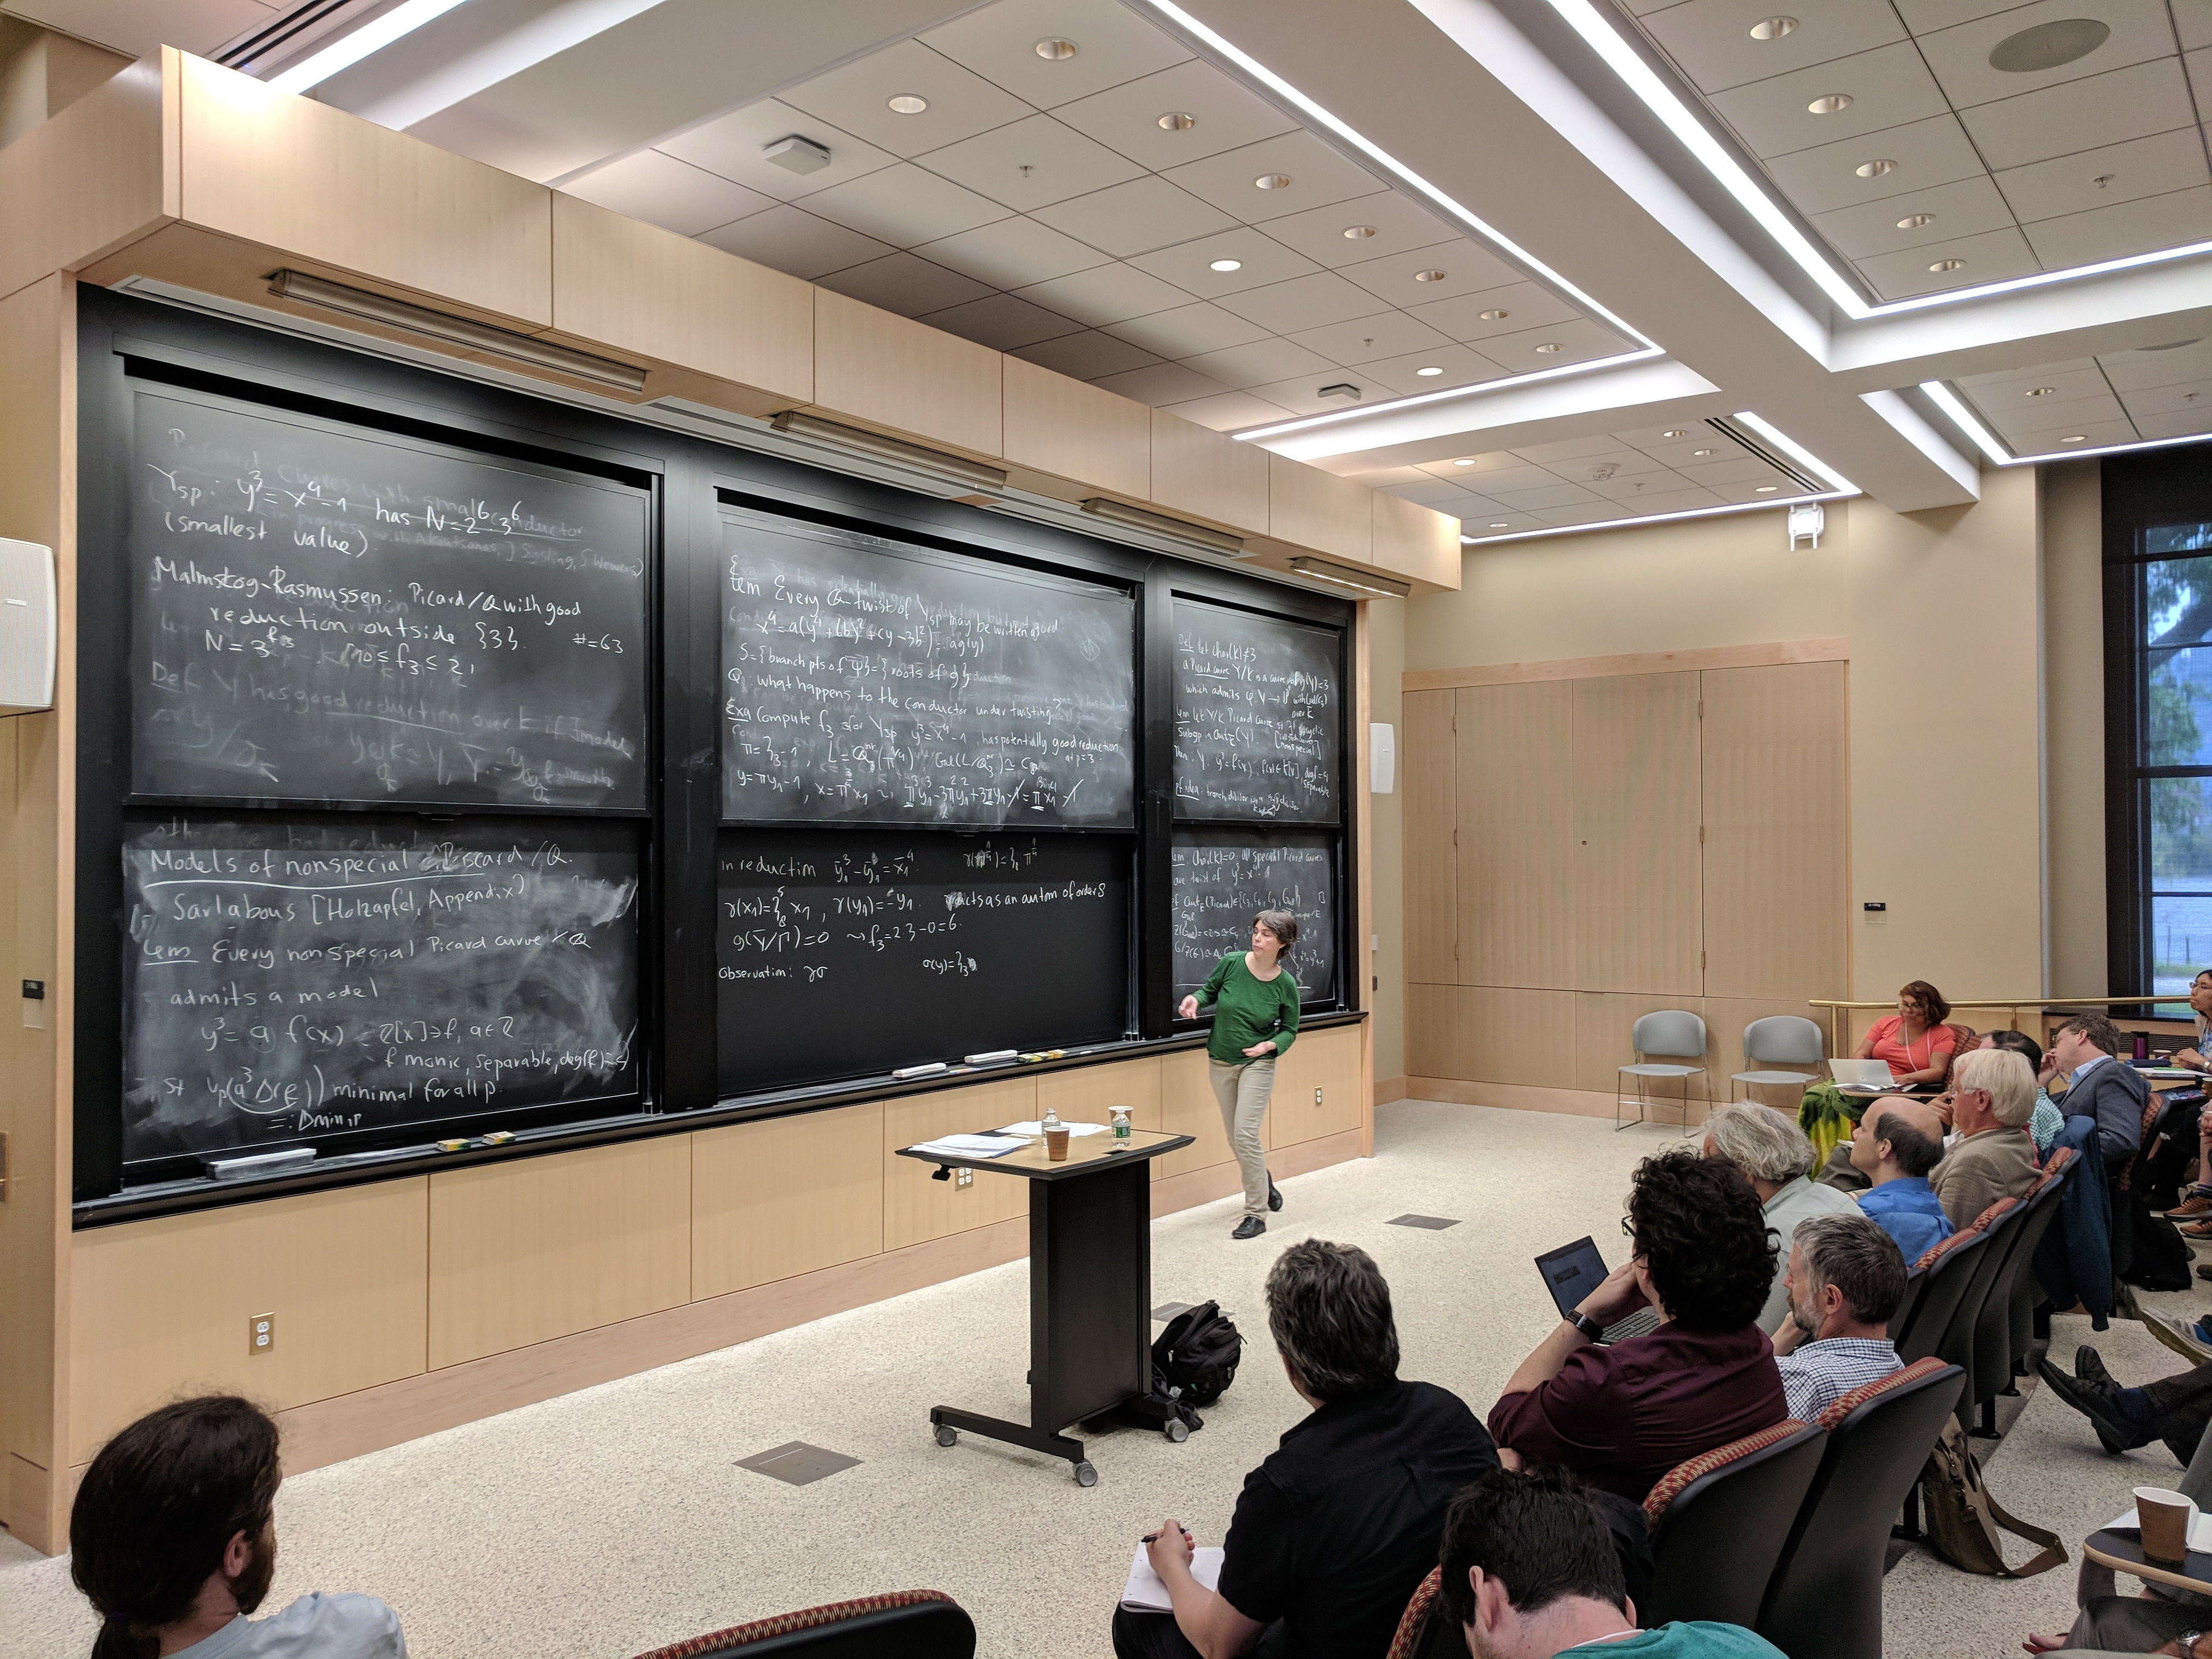
\includegraphics[width=0.95\textwidth]{conference-drew2018}

  Fragen sind während des gesamten Vortrags willkommen. \\
  Bitte keinesfalls bis zum Ende aufsparen. \\
  Vielen Dank dafür! $\heartsuit$
  \par
\end{frame}

\section{Ordinalzahlen}
\only<2>{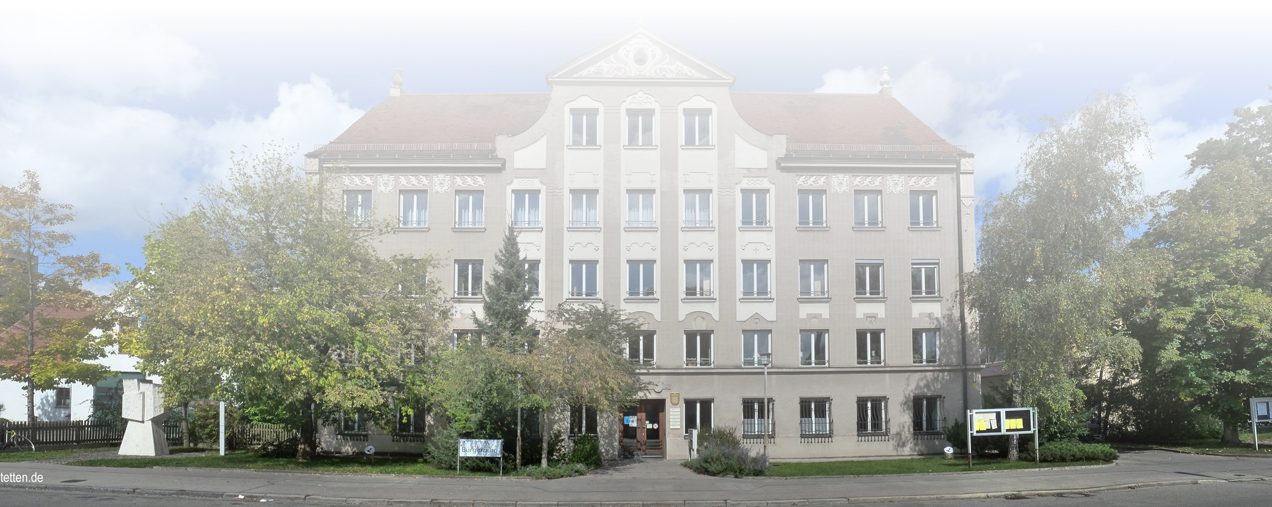
\includegraphics[width=\paperwidth]{buergerbuero-haunstetten}}

% https://commons.wikimedia.org/wiki/File:RathausKoenigsbrunn.jpg
{\usebackgroundtemplate{\begin{minipage}{\paperwidth}\vspace*{1cm}\includegraphics[width=\paperwidth]{rathaus-koenigsbrunn}\end{minipage}}
\begin{frame}
  \centering
  \bigskip

  \Huge \hil{Teil I}

  \bigskip
  \Large\textbf{Ordinalzahlen}
  \par

  messen Anordnung
  \par
\end{frame}}

{\usebackgroundtemplate{\begin{minipage}{\paperwidth}\vspace*{5cm}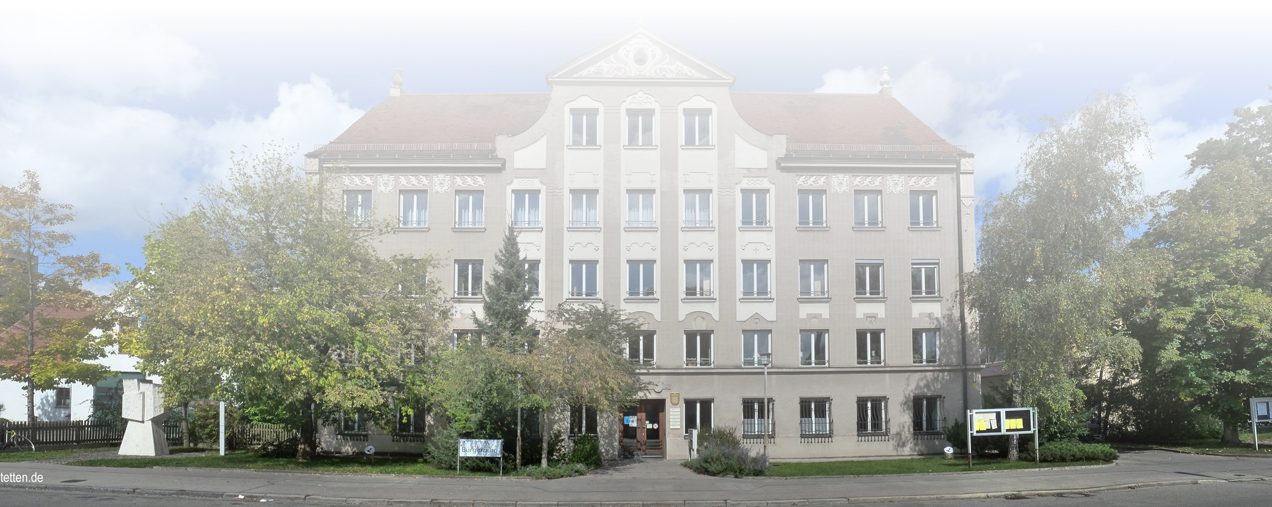
\includegraphics[width=\paperwidth]{buergerbuero-haunstetten}\end{minipage}}
\begin{frame}
  \centering
  \bigskip

  \Huge \hil{Teil I}

  \bigskip
  \Large\textbf{Ordinalzahlen}
  \par

  messen Anordnung
  \par
\end{frame}}


\begin{frame}
  \centering
  \bigskip

  \Huge \hil{Was nun?}
  \bigskip
  \bigskip

  \large

  \begin{itemize}\justifying
    \item Wozu sind unendlich große Zahlen gut? \\ Herkulas Kampf gegen die Hydra
    \bigskip
    \item Eine andere Geschmacksrichtung von Unendlichkeit und unkennbare
    Antworten
    \bigskip
    \item Ein transfinites Spiel, das ihr verlieren werdet
  \end{itemize}

  \bigskip
\end{frame}

\section{Kardinalzahlen}

\begin{frame}
  \centering
  \bigskip

  \Huge \hil{Teil II}

  \bigskip
  \Large\textbf{Kardinalzahlen}
  \par

  messen Anzahl
  \par
  \bigskip
  \bigskip

  \only<1>{
    \begin{columns}[t]
      \begin{column}{0.2\textwidth}\end{column}
      \begin{column}{0.3\textwidth}
        \centering
        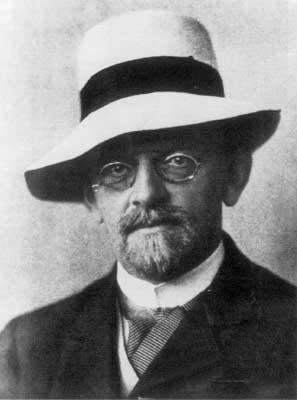
\includegraphics[height=0.33\textheight]{hilbert} \\
        {\scriptsize David Hilbert \\ * 1862 \\ † 1943\par}
      \end{column}
      \begin{column}{0.3\textwidth}
        \centering
        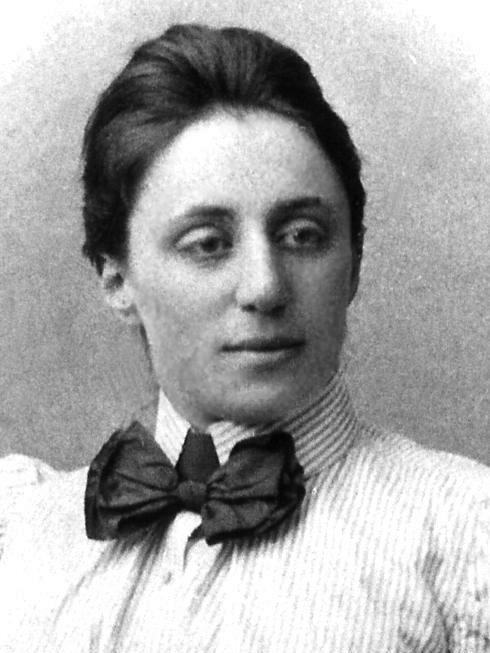
\includegraphics[height=0.33\textheight]{noether} \\
        {\scriptsize Emmy Noether \\ * 1882 \\ † 1935\par}
      \end{column}
      \begin{column}{0.2\textwidth}\end{column}
    \end{columns}
  }

  \raggedright
  \only<2->{\begin{columns}[b]
    \begin{column}{0.05\textwidth}\end{column}
    \begin{column}{0.65\textwidth}
      \visible<3->{Es gibt \hil{$\boldsymbol{\aleph_0}$} viele natürliche Zahlen: 1, 2, 3, \ldots}
      \bigskip

      \visible<4->{$\aleph_0 + 1 = \aleph_0$}
      \bigskip

      \visible<5->{$\aleph_0 \cdot \aleph_0 = \aleph_0$}
    \end{column}
    \begin{column}{0.45\textwidth}
      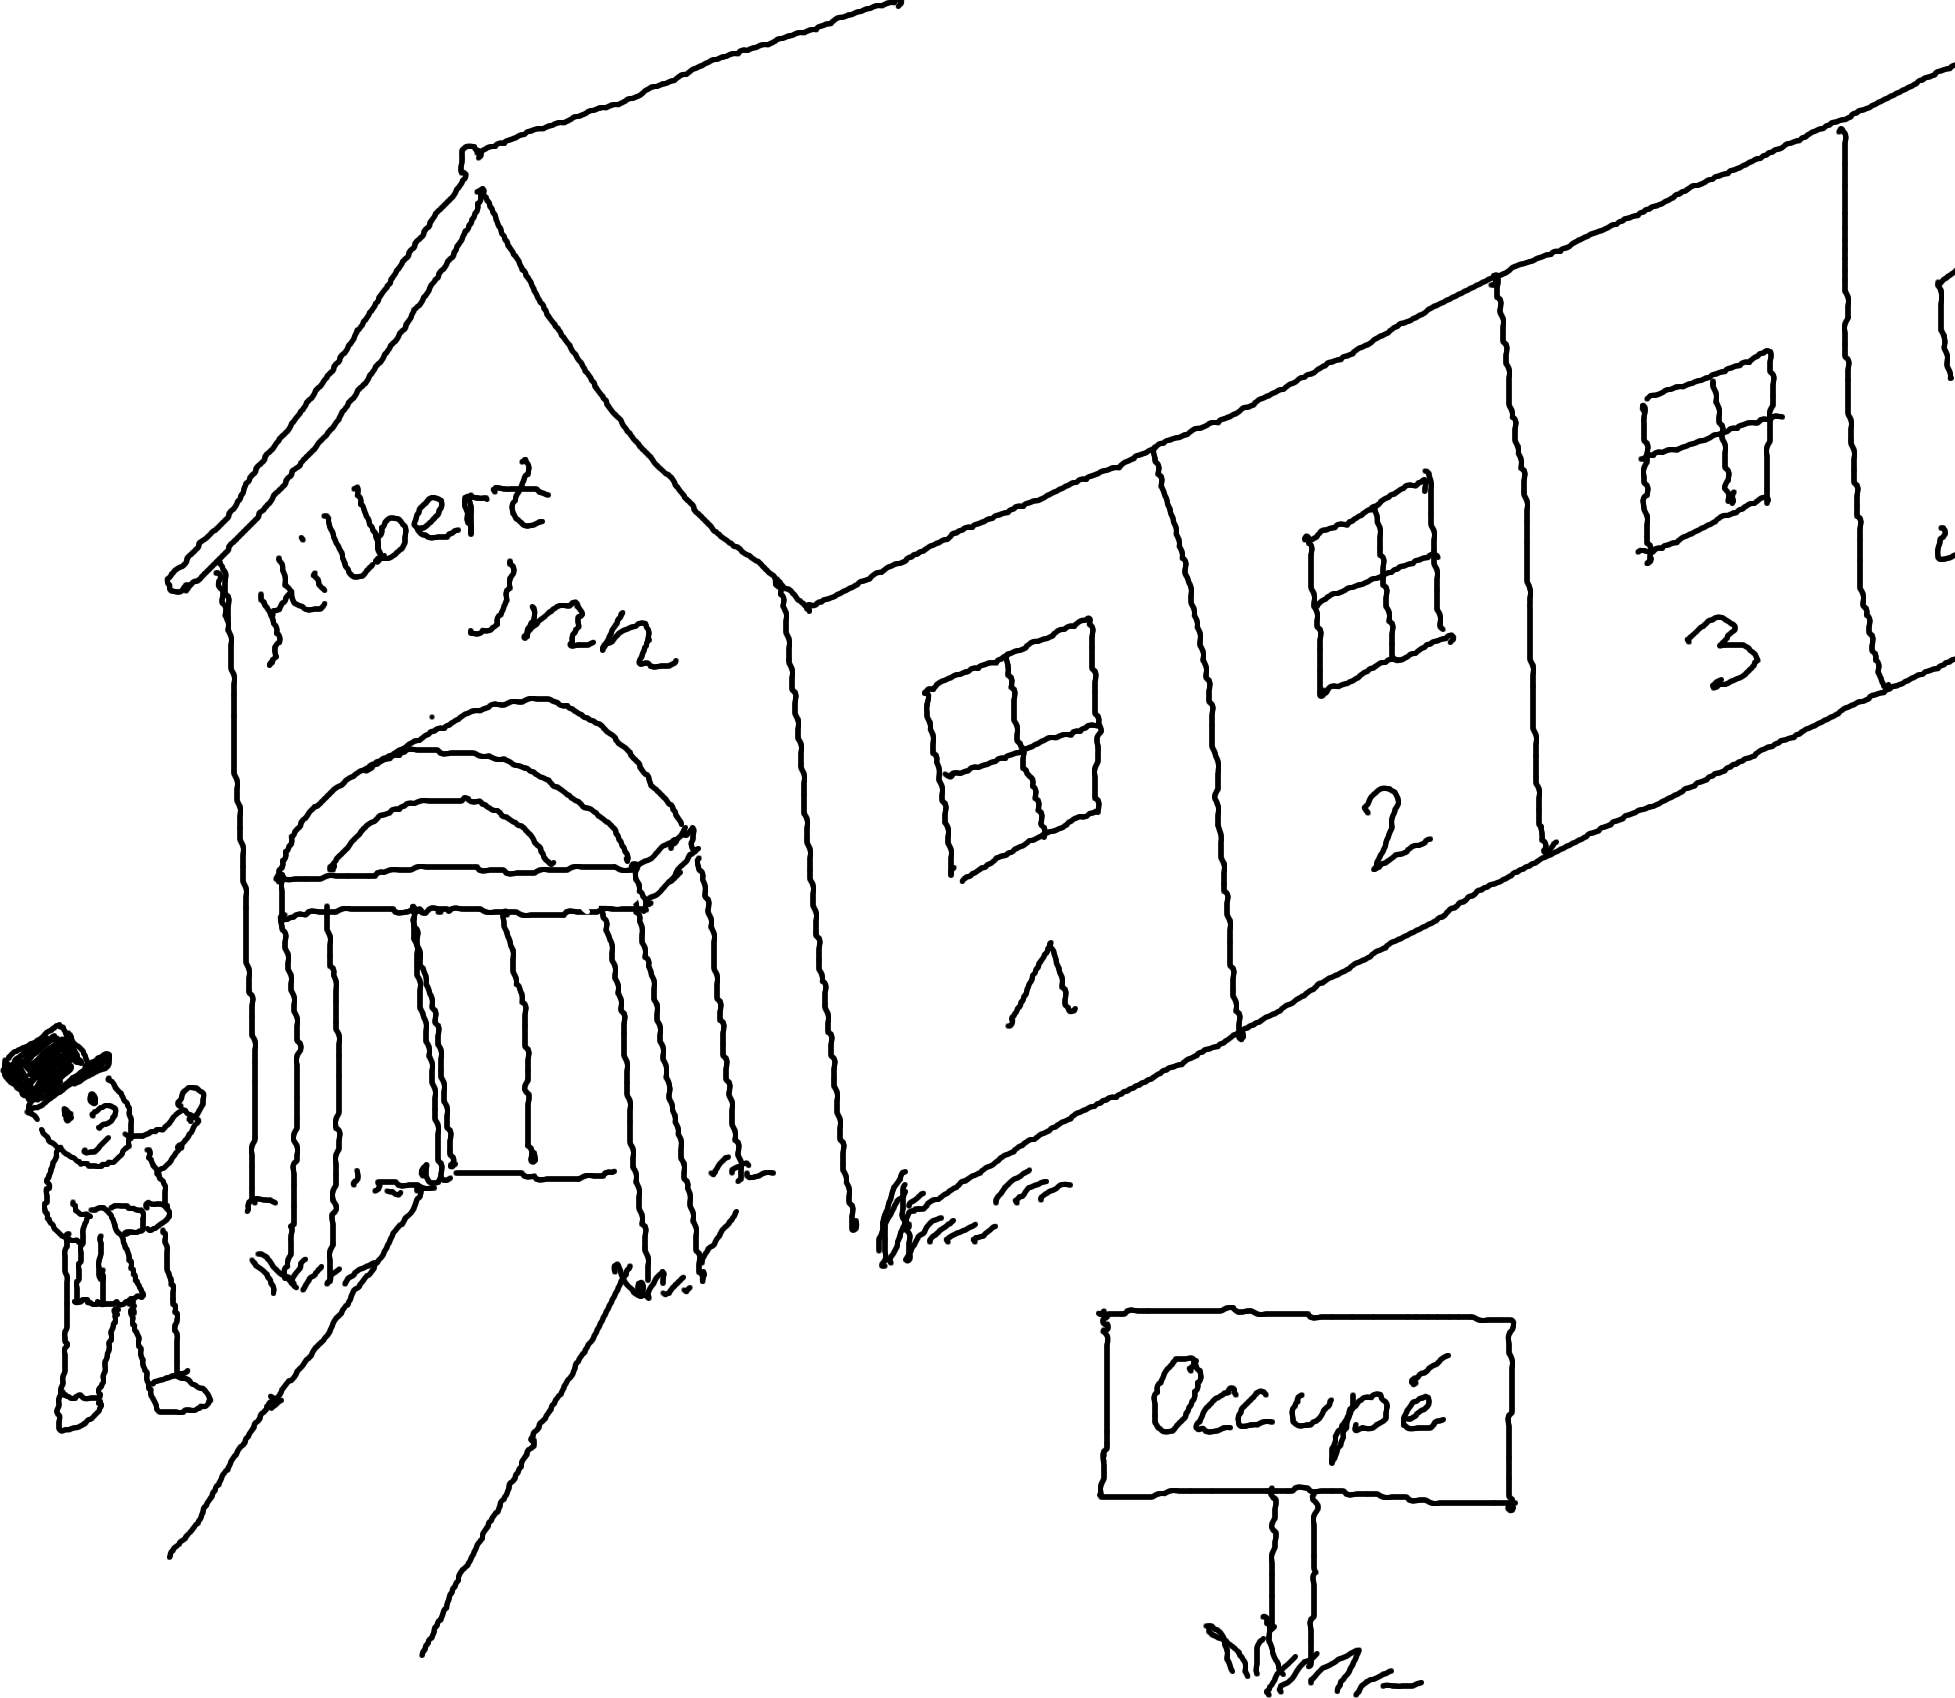
\includegraphics[width=5.5cm]{hilberts-hotel}
      \vspace*{-0.4cm}
    \end{column}
  \end{columns}}
\end{frame}

\begin{frame}{Größen wichtiger Mengen}
  \begin{itemize}
    \item Es gibt~\hil{$\boldsymbol{\aleph_0}$} viele \hil{natürliche Zahlen}.

    \begin{center}\begin{tikzpicture}
      \draw[color=white] (-3.5,0) -- (1,0);
      \draw[-latex,dotted] (1.0,0) -- (3.5,0);
      \foreach \x in {1,2,3}
      \draw[shift={(\x,0)},color=black] (0pt,3pt) -- (0pt,-3pt);
      \foreach \x in {1,2,3}
      \draw[shift={(\x,0)},color=black] (0pt,0pt) -- (0pt,-3pt) node[below] {$\x$};
    \end{tikzpicture}\end{center}
    \pause

    \item Es gibt auch nur \hil{$\boldsymbol{\aleph_0}$} viele \hil{ganze Zahlen}.

    \begin{center}\begin{tikzpicture}
      \draw[latex-latex,dotted] (-3.5,0) -- (3.5,0);
      \foreach \x in {-3,-2,-1,0,1,2,3}
      \draw[shift={(\x,0)},color=black] (0pt,3pt) -- (0pt,-3pt);
      \foreach \x in {-3,-2,-1,0,1,2,3}
      \draw[shift={(\x,0)},color=black] (0pt,0pt) -- (0pt,-3pt) node[below] {$\x$};
    \end{tikzpicture}\end{center}
    \pause

    \item Ebenso gibt es nur \hil{$\boldsymbol{\aleph_0}$} viele
    \hil{rationale Zahlen}.

    \begin{center}\begin{tikzpicture}
      \draw[latex-latex,densely dotted] (-3.5,0) -- (3.5,0);
      \foreach \x in {-3,-2,-1,0,1,2,3,1.5,2.3333}
      \draw[shift={(\x,0)},color=black] (0pt,3pt) -- (0pt,-3pt);
      \foreach \x in {-3,-2,-1,0,1,2,3}
      \draw[shift={(\x,0)},color=black] (0pt,0pt) -- (0pt,-3pt) node[below] {$\x$};
      \draw[shift={(1.5,0)},color=black] (0pt,0pt) -- (0pt,-3pt) node[below]
      {\scriptsize $\frac{3}{2}$};
      \draw[shift={(2.3333,0)},color=black] (0pt,0pt) -- (0pt,-3pt) node[below]
      {\scriptsize $2\frac{1}{3}$};
    \end{tikzpicture}\end{center}
    \pause

    \item Aber es gibt \hil{mehr} reelle Zahlen:
    \hil{$\boldsymbol{\mathfrak{c}}$} viele.

    \begin{center}\begin{tikzpicture}
      \draw[latex-latex] (-3.5,0) -- (3.5,0);
      \foreach \x in {-3,-2,-1,0,1,2,3,1.4142,3.141592}
      \draw[shift={(\x,0)},color=black] (0pt,3pt) -- (0pt,-3pt);
      \foreach \x in {-3,-2,-1,0,1,2,3}
      \draw[shift={(\x,0)},color=black] (0pt,0pt) -- (0pt,-3pt) node[below] {$\x$};
      \draw[shift={(1.4142,0)},color=black] (0pt,0pt) -- (0pt,-3pt) node[below] {\scriptsize $\sqrt{2}$};
      \draw[shift={(3.141592,0)},color=black] (0pt,0pt) -- (0pt,-3pt) node[below] {\scriptsize $\pi$};
    \end{tikzpicture}\end{center}
  \end{itemize}
\end{frame}


\section{Erkenntnistheorie}

\begin{frame}
  \centering
  \bigskip

  \Huge \hil{Teil III}

  \bigskip
  \Large\textbf{Erkenntnistheorie}
  \par
  \normalsize
  \bigskip
  \bigskip
  \bigskip
  \bigskip

  \begin{columns}[t]
    \begin{column}{0.32\textwidth}
      \centering\includegraphics[width=0.7\textwidth]{p-adic-numbers}
      \medskip

      "`Es gibt unendlich viele Primzahlen."'
    \end{column}
    \begin{column}{0.32\textwidth}
      \centering\includegraphics[width=0.9\textwidth]{platonic-solids}
      \medskip

      "`Es gibt nur fünf platonische Körper."'
    \end{column}
    \begin{column}{0.37\textwidth}
      \centering\includegraphics[width=0.7\textwidth]{hafez-tomb}
      \medskip

      "`Der goldene Schnitt ist die irrationalste Zahl."'
    \end{column}
  \end{columns}
\end{frame}

\begin{frame}{Die Kontinuumshypothese}
  \begin{columns}[t]
    \begin{column}{0.34\textwidth}
      \centering\includegraphics[height=0.5\textheight]{georg-cantor} \\
      {\scriptsize Georg Cantor (* 1845, † 1918)\par}
      \bigskip

      Gibt es eine Zwischenstufe zwischen $\aleph_0$ und $\mathfrak{c}$?
    \end{column}
    \pause

    \begin{column}{0.34\textwidth}
      \centering\includegraphics[height=0.5\textheight]{kurt-goedel} \\
      {\scriptsize Kurt Gödel (* 1906, † 1978)\par}
      \bigskip

      Es gibt keinen Beweis, dass es eine Zwischenstufe gibt.
    \end{column}
    \pause

    \begin{column}{0.34\textwidth}
      \centering\includegraphics[height=0.5\textheight]{paul-cohen} \\
      {\scriptsize Paul Cohen (* 1934, † 2007)\par}
      \bigskip

      Es gibt keinen Beweis, dass es keine Zwischenstufe gibt.
    \end{column}
  \end{columns}
\end{frame}


\section*{}

\begin{frame}
  \centering
  \bigskip

  \Huge \hil{Abschluss}
  \bigskip

  \normalsize
  \raggedright

  \begin{itemize}
    \item Ordinalzahlen messen Anordnung.
    $\omega + 1 > \omega$

    \item Kardinalzahlen messen Anzahl.
    $\aleph_0 + 1 = \aleph_0$

    \item Es gibt mathematische Fragen, deren Antwort bewiesenermaßen dauerhaft
    unkennbar ist.
  \end{itemize}
  \pause
  \bigskip

  \centering
  \hil{Mathecamp vom 17. bis 25. August in Violau}
  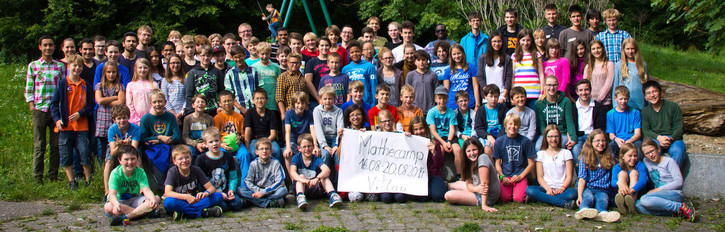
\includegraphics[width=\textwidth]{mathecamp-gruppenfoto-klein}
\end{frame}

\end{document}

% Grab des Hafez in Shiraz (Iran), Aufnahme von Pentocelo
% Kontinuumshypothese: Aussage, dass es keine Zwischenstufe gibt.
% Cantors Begründung der Mengenlehre: 1874 bis 1897
% Cantors Vermutung: 1878
% Gödels Beweis: 1938
% Cohens Beweis: 1963
% Protagoras: möglicherweise * 490 v. Chr., † 411 v. Chr.
